This last section shows the characterization of the active shield (cosmic veto), the physical configuration of which was explained in section \ref{subsec:SetUpActiveShield}. This characterization was carried out using PMTs as photosensors as shown in Figure \ref{fig:VetoAndPrototype}, which are readout using the electronic configuration shown in section \ref{subsubsec:PMTsElectronicalSystem}, Figure \ref{subfig:ElectronicConfiguraiton4PMT}. Measurements of the cosmic veto using SiPM arrays has already started and their replacement will be as soon as possible. 

First of all, we have to find the conditions in which the detection of cosmic events will be optimized by our active veto. It consists of, on the one hand, finding the minimum high voltage of PMTs in which their efficiency is stable, and, on the other hand, finding the maximum threshold of the discriminator, which has to be overcomed by the output signals of the PMTs to contribute to the cosmic detection, at which we start to loss cosmic events in their detection. For higher high voltage and smaller thresholds of the found values, a plateau should be found.

To find both parameters, several measures of the number of coincident events (cosmic events) were done. On the one hand it was measured at several high voltages and fixed thresholds and on the other hand it was measured at several thresholds and fixed high voltages. Both measurements are shown in Figure \ref{fig:HVandThresholdsPLateaus} in which a semi-logarithmic scale has been used.

A modification of the electron configuration has been made only for finding these optimal conditions, which consists of using the electronic configuration shown in Figure \ref{subfig:ElectronicConfiguraiton4PMT} where the amplification part has been eliminated and the output signal of the coincidence module, second stage, is connected to a CAEN Quad Scaler And Preset Counter-Timer module, N. 1145, \cite{ScalerDataSheet}, which is used to count the number of events in a time window ($300$ seconds in our case).

\begin{figure}[]
 \centering
  \subfloat[Counts per second for several high voltage at three different thresholds.]{
   \label{subfig:HVPLateauVetos}
    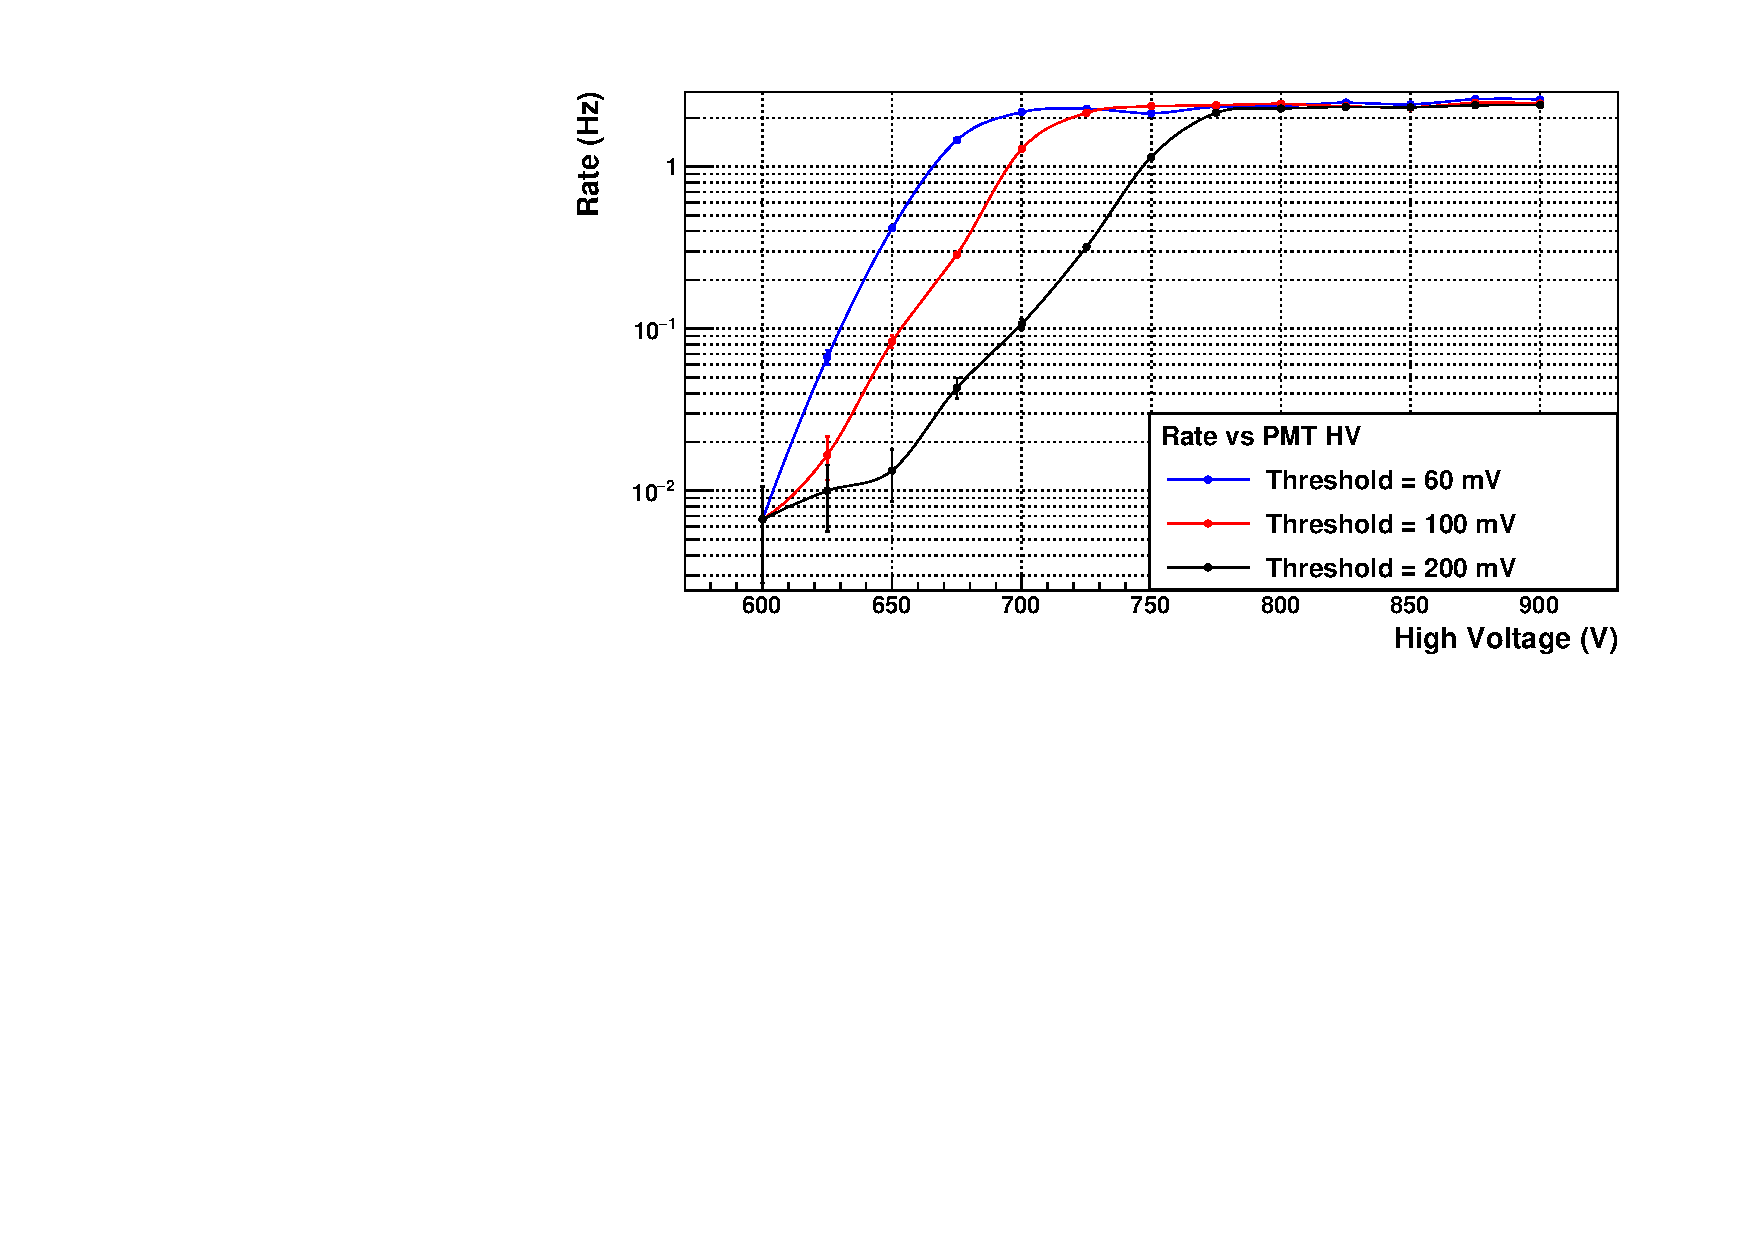
\includegraphics[width=0.8\textwidth]{4ResearchAndDevelopments/43CosmicVetos/Counts_for_several_HV_VETOS.pdf}}
    \newline
  \subfloat[Counts per second for several thresholds at three different high voltage.]{
   \label{subfig:ThresholdsPlateau}
    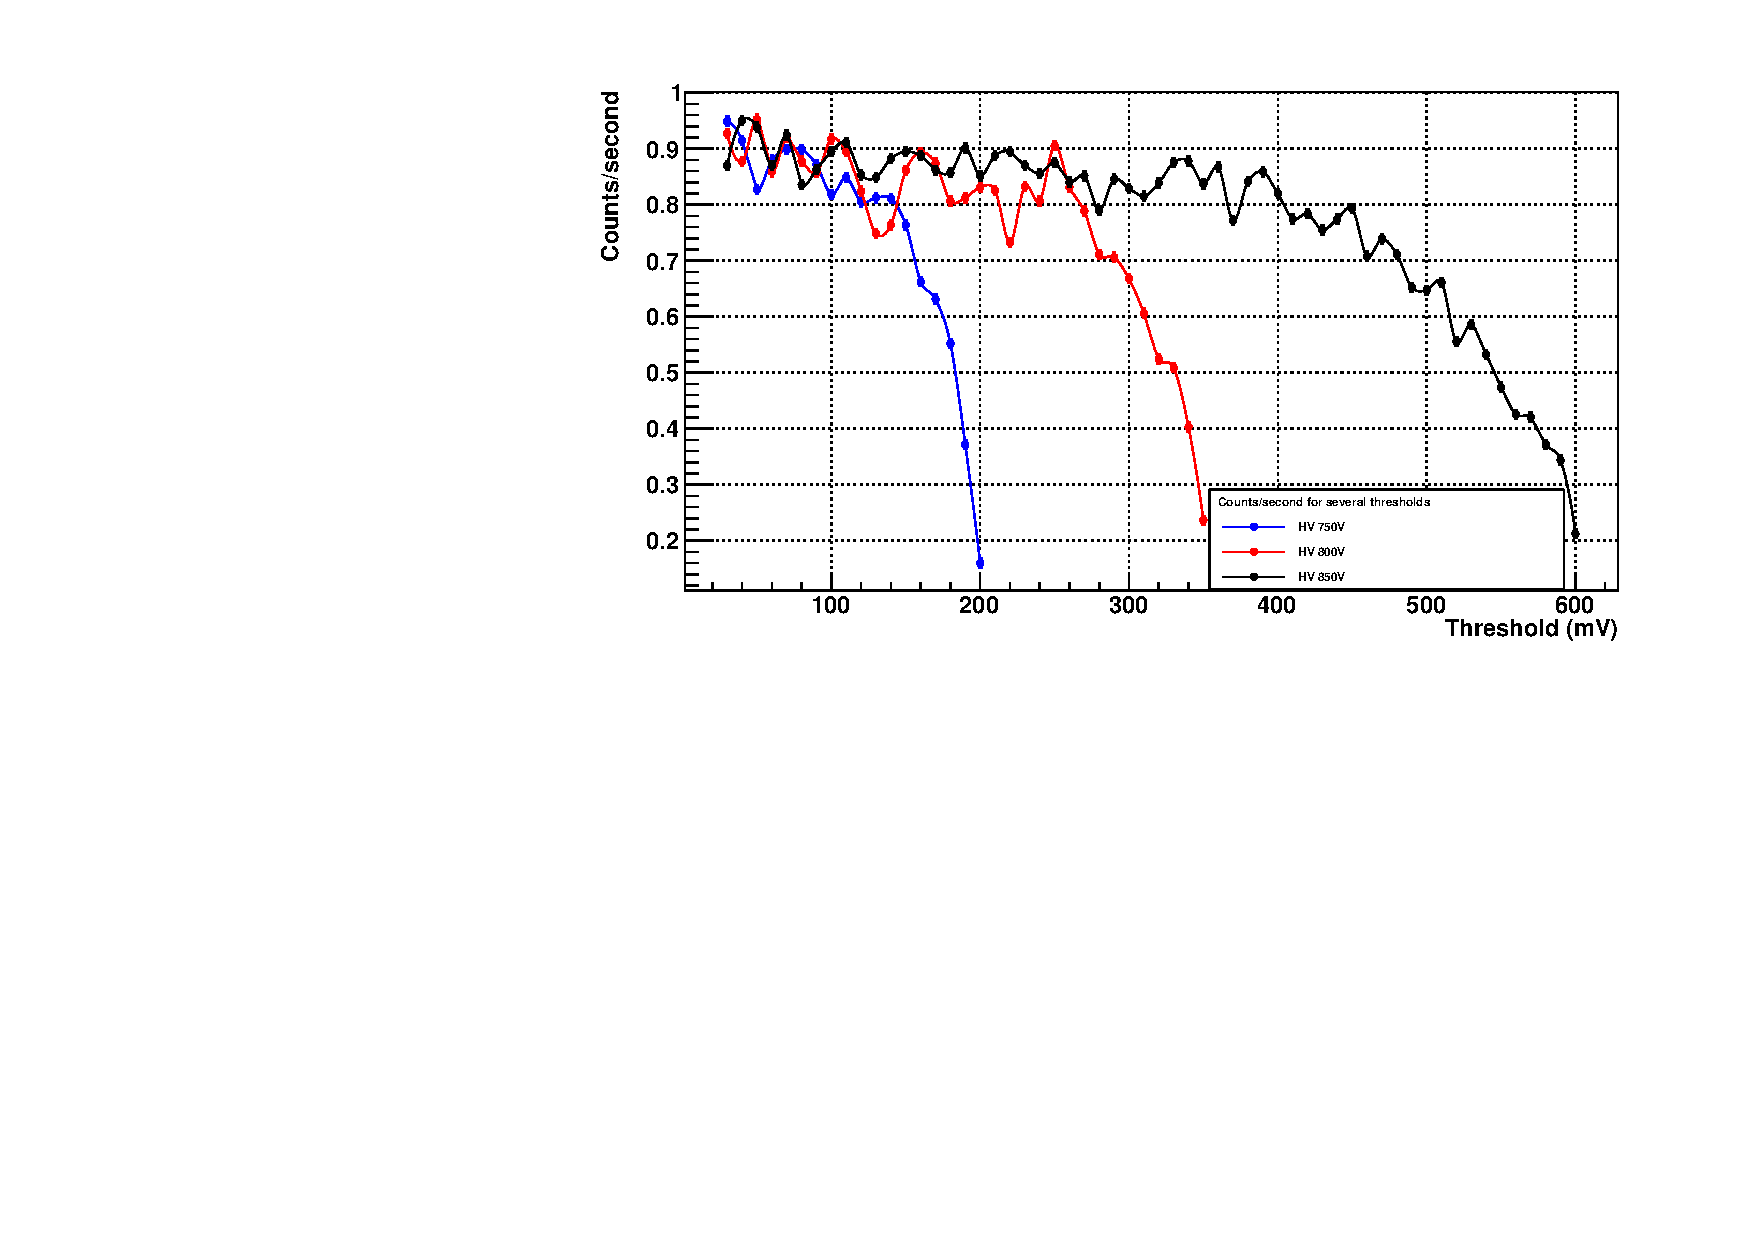
\includegraphics[width=0.8\textwidth]{4ResearchAndDevelopments/43CosmicVetos/Counts_for_several_thresholds_VETOS.pdf}}
 \caption{Counts per second at several high voltage and fixed thresholds and several thresholds and fixed high voltage.}
 \label{fig:HVandThresholdsPLateaus}
\end{figure}

In Figure \ref{subfig:HVPLateauVetos}, the measurements at several high voltage and a fixed thresholds is shown, which have been done for three different thresholds, $60~\milli\volt$, $100~\milli\volt$ and $200~\milli\volt$. As can be seen, there is a minimum high voltage for each threshold used, $700~\volt$, $730~\volt$ and $780~\volt$ respectively, at which the plateau start. As we can see this minimum voltage is higher when we increase the value of the threshold, as we should hope. The voltage chosen to work is $800~\volt$ since we can be sure of being on the plateau for the three thresholds.

In the same way, in Figure \ref{subfig:ThresholdsPlateau}, the measurements at several thresholds and a fixed high voltage is shown, which have been done for three different high voltages, $750~\volt$, $800~\volt$ and $850~\volt$. As can be seen, there is a maximum threshold for each high voltage used,  $140~\milli\volt$, $270~\milli\volt$ and $450~\milli\volt$ respectively, at which the plateau ends. Now, we can see that this maximum threshold is increased for higher voltage, as we should hope. The threshold choosen to work is $200~\milli\volt$ since, for our last election $800~\volt$, we can be sure of being on the plateau. 

Next, the energy spectrum of cosmic events was measured, which is shown in Figure \ref{fig:EnergySpectrumCosmicVeto}. For this task the electronic configuration shown in Figure \ref{subfig:ElectronicConfiguraiton4PMT} was used with the values previously mentioned, $800~\volt$ and $200~\milli\volt$. 

\begin{figure}[h]
\centering
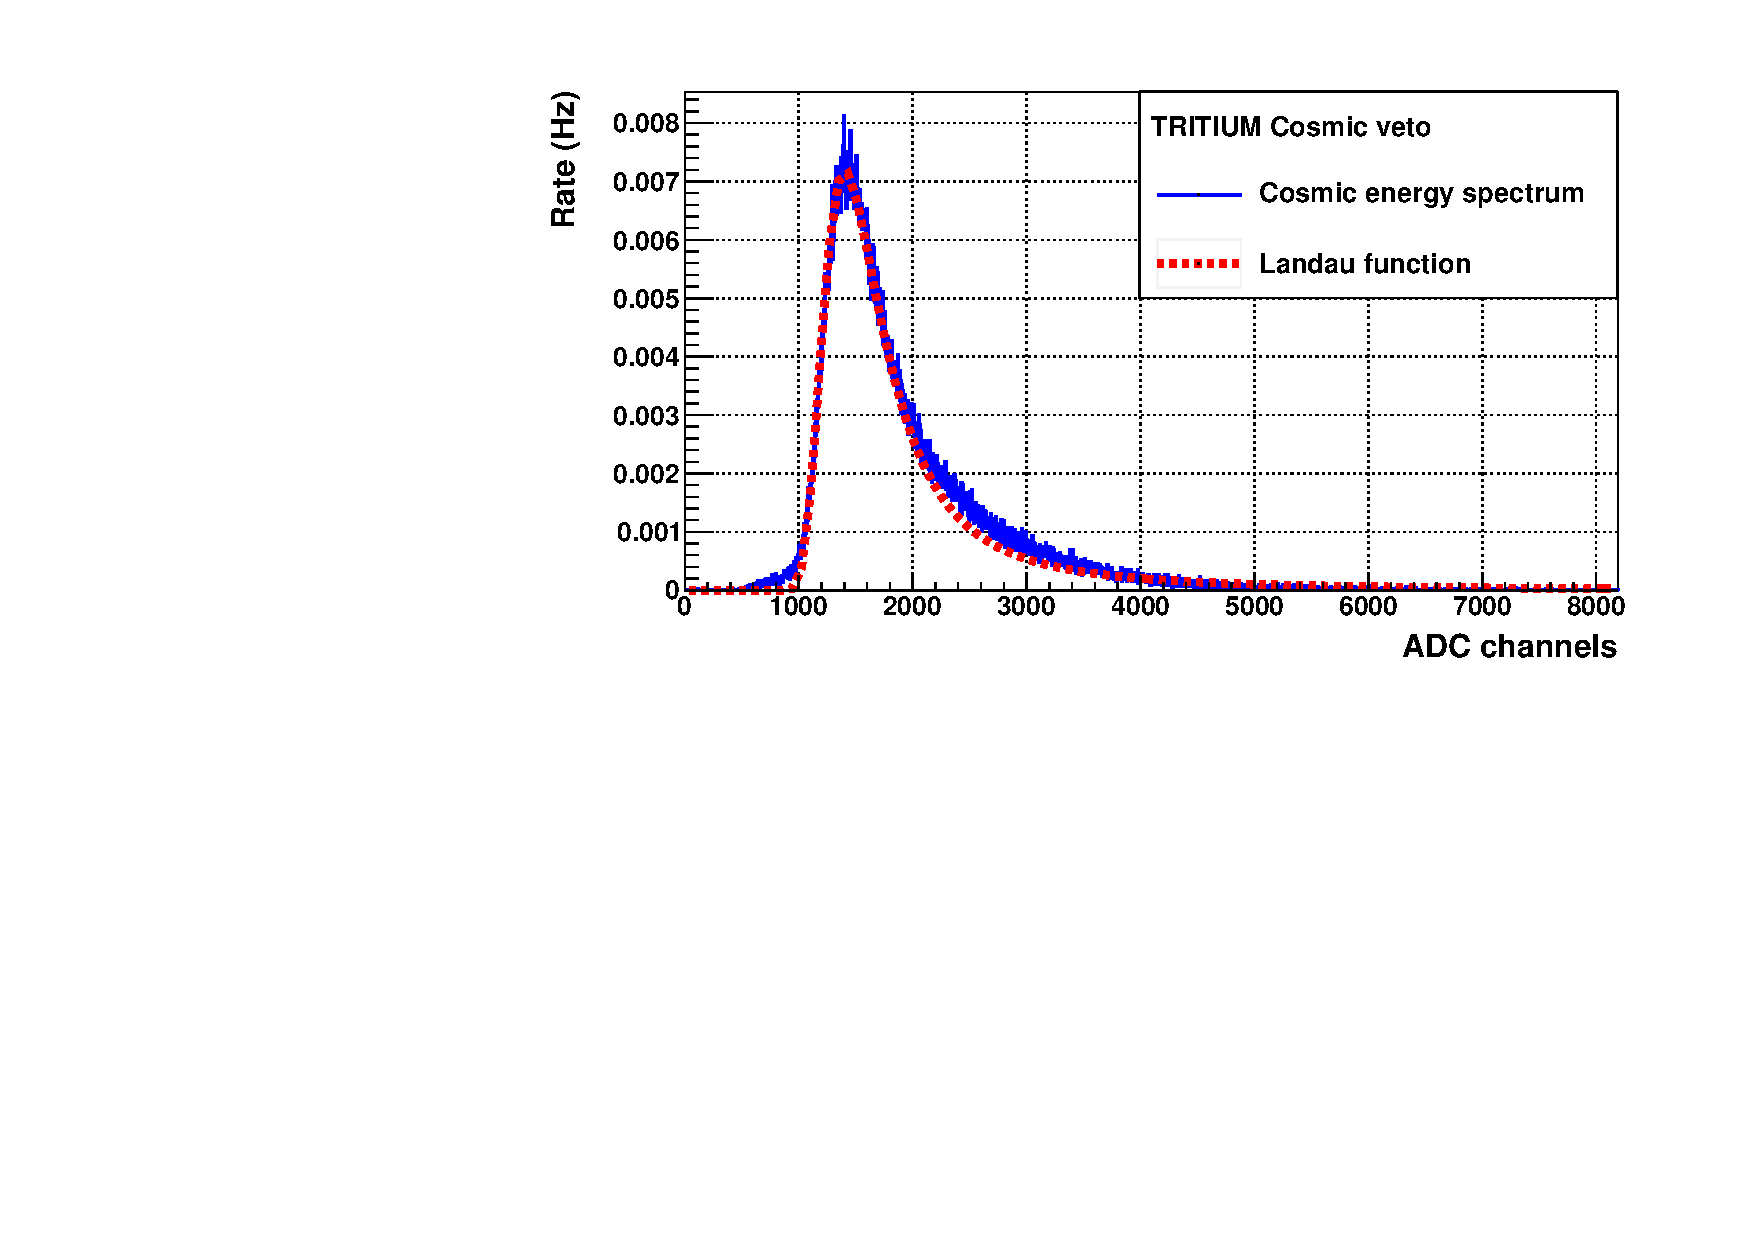
\includegraphics[scale=0.6]{4ResearchAndDevelopments/43CosmicVetos/Cosmic_Energy_Spectrum_36_cm_Landau_Function.pdf}
\caption{Energy spectrum measured with the cosmic veto.\label{fig:EnergySpectrumCosmicVeto}}
\end{figure}

As we can see, this energy spectrum fits well with a landau function as expected. Now, the number of detected cosmic events can be known by calculating the area integral of this spectrum, whose result is $2,5~$event$/\second$. The theoretically expected cosmic rate was calculated in section \ref{subsec:SetUpActiveShield} for our cosmic vetos, $2,909~$event$/\second$, so the efficiency of it for cosmic events can be calculated, whose value is $85\%$, which is a common value of the efficiency of this type of detectors.

Finally the relationship between the detected cosmic events and the distance between both detectors that form the cosmic veto was obtained. It is interesting because this distance can be changed if other tritium prototypes are used and we need to know the expected cosmic rate for each different situation.

To do so, an energy spectrum was measured for five different distances, $10.4~\cm$, $20~\cm$, $36~\cm$, $39.8~\cm$ and $50~\cm$, which is shown in Figure \ref{fig:EnergySpectrumsSeveralDistanceVeto}. The energy spectrum previously shown in Figure \ref{fig:EnergySpectrumCosmicVeto} was also included. 

\begin{figure}[h]
\centering
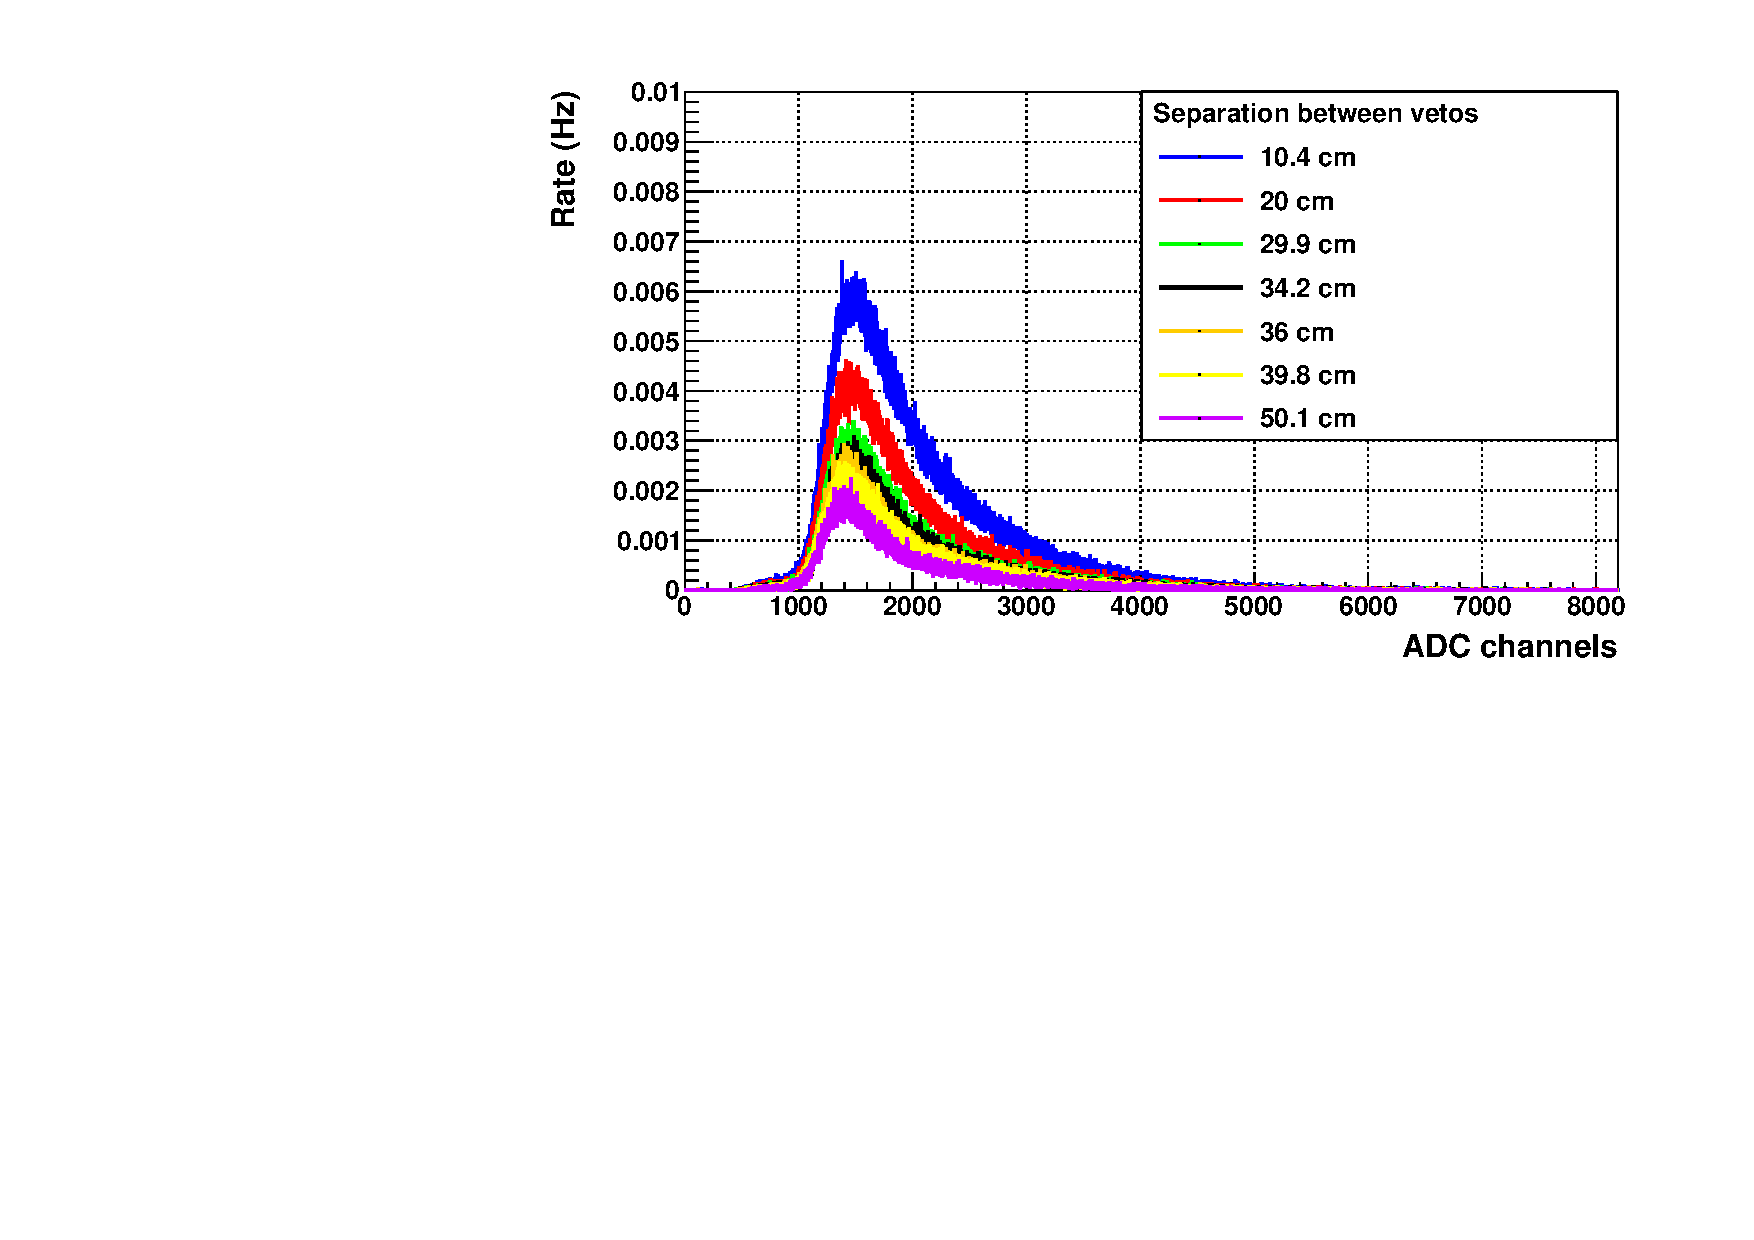
\includegraphics[scale=0.6]{4ResearchAndDevelopments/43CosmicVetos/Energy_Plots_SeveralDistance_Veto.pdf}
\caption{Energy spectrum of cosmic vetos for several distance between cosmic detectors.\label{fig:EnergySpectrumsSeveralDistanceVeto}}
\end{figure}

As we can see, the shape of the spectrum is the same because the energy of the detected events is the same (cosmic events) but the quantity of their events is less for greater distance. The reason for that is that when we increase the distance, the solid angle formed by the active veto is smaller.

The detected cosmic events was calculated by the area integral and they are represented in Figure \ref{fig:LinearFitSeveralDistanceVeto} where a linear fit has been added. With this linear fit, the detected cosmic rate can be easily known whatever the working distance. 

\begin{figure}[h]
\centering
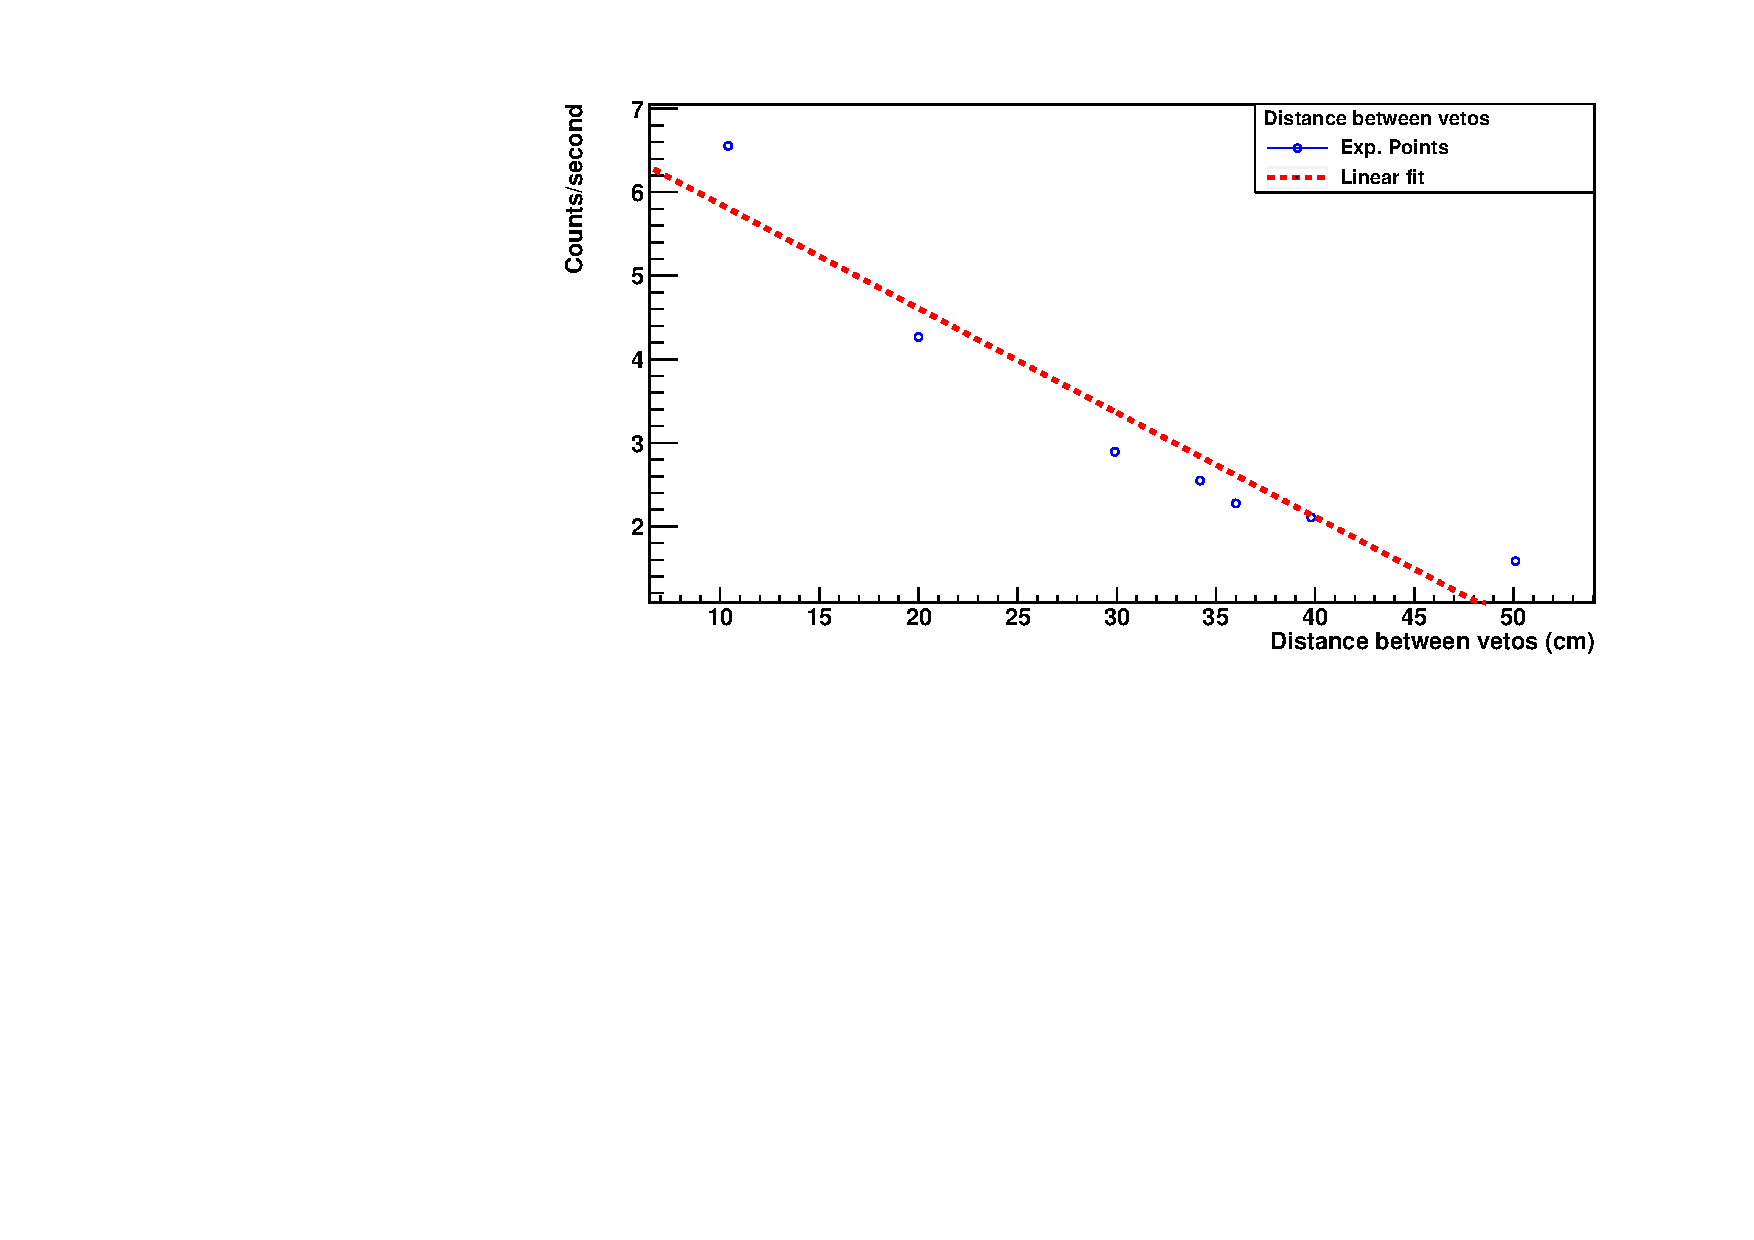
\includegraphics[scale=0.6]{4ResearchAndDevelopments/43CosmicVetos/LinearFit_SeveralDistance_Veto.pdf}
\caption{Linear fit of the counts per second measured with the cosmic veto with several distance between its cosmic detectors.\label{fig:LinearFitSeveralDistanceVeto}}
\end{figure}



Falta poner la medida antes y despues de cubrir el detector.

También se realizaron varias medias para ver como afecta una fuente gama. Discutir con Pepe como plantear esta medida o si merece la pena ponerla o no.

Como es de esperar esta deja muy poca señal en el centelleador ya que este tiene muy poca eficiencia para gammas.